\documentclass[12pt, a4paper, oneside, openright, titlepage]{book}
\usepackage[utf8]{inputenc}
\raggedbottom
\usepackage{import}


%%%%%%%%%%%%%%%%% Book Formatting Comments:

%%%%%%%%%%%%%%%%%%%%%%%%%%%%%%%%%%%%% for Part

%%%%%%%%%%%%%%%%%%%%%% for chapter

%%%%%%%%%%%%%%%%%%%% for section








%%%%%% PACKAGES %%%%%%%
\usepackage{hyperref}
\hypersetup{
    colorlinks,
    citecolor=black,
    filecolor=black,
    linkcolor=black,
    urlcolor=black
}
\usepackage{amsmath} % Math display options
\usepackage{amssymb} % Math symbols
\usepackage{amsfonts} % Math fonts
\usepackage{amsthm}
\usepackage{mathtools} % General math tools
\usepackage{array} % Allows you to write arrays
\usepackage{empheq} % For boxing equations
\usepackage{mathabx}
\usepackage{mathrsfs}
\usepackage{nameref}

\usepackage{soul}
\usepackage[normalem]{ulem}

\usepackage{txfonts}
\usepackage{cancel}
\usepackage[toc, page]{appendix}
\usepackage{titletoc,tocloft}
\setlength{\cftchapindent}{1em}
\setlength{\cftsecindent}{2em}
\setlength{\cftsubsecindent}{3em}
\setlength{\cftsubsubsecindent}{4em}
\usepackage{titlesec}

\titleformat{\section}
  {\normalfont\fontsize{25}{15}\bfseries}{\thesection}{1em}{}
\titleformat{\section}
  {\normalfont\fontsize{20}{15}\bfseries}{\thesubsection}{1em}{}
\setcounter{secnumdepth}{1}  
  
  

\newcommand\numberthis{\refstepcounter{equation}\tag{\theequation}} % For equation labelling
\usepackage[framemethod=tikz]{mdframed}

\usepackage{tikz} % For drawing commutative diagrams
\usetikzlibrary{cd}
\usetikzlibrary{calc}
\tikzset{every picture/.style={line width=0.75pt}} %set default line width to 0.75p

\usepackage{datetime}
\usepackage[margin=1in]{geometry}
\setlength{\parskip}{1em}
\usepackage{graphicx}
\usepackage{float}
\usepackage{fancyhdr}
\setlength{\headheight}{15pt} 
\pagestyle{fancy}
\lhead[\leftmark]{}
\rhead[]{\leftmark}

\usepackage{enumitem}

\usepackage{url}
\allowdisplaybreaks

%%%%%% ENVIRONMENTS %%%
\definecolor{purp}{rgb}{0.29, 0, 0.51}
\definecolor{bloo}{rgb}{0, 0.13, 0.80}



%%\newtheoremstyle{note}% hnamei
%{3pt}% hSpace above
%{3pt}% hSpace belowi
%{}% hBody fonti
%{}% hIndent amounti
%{\itshape}% hTheorem head fonti
%{:}% hPunctuation after theorem headi
%{.5em}% hSpace after theorem headi
%{}% hTheorem head spec (can be left empty, meaning ‘normal’)i


%%%%%%%%%%%%% THEOREM STYLES

\newtheoremstyle{BigTheorem}
{20pt}
{20pt}
{\slshape}
{}
{\Large\color{purp}\bfseries}
{.}
{\newline}
{\thmname{#1}\thmnumber{ #2}\thmnote{ (#3)}}



\newtheoremstyle{TheoremClassic}
{15pt}
{15pt}
{\slshape}
{}
{\bfseries}
{.}
{.5em}
{}

\newtheoremstyle{Definitions}
{15pt}
{15pt}
{\slshape}
{}
{\bfseries}
{.}
{.5em}
{\thmname{#1}\thmnumber{ #2}\thmnote{ (#3)}}


\newtheoremstyle{Remarks}
{10pt}
{10pt}
{\upshape}
{}
{\bfseries}
{.}
{.5em}
{}

\newtheoremstyle{Examples}
{10pt}
{10pt}
{\upshape}
{}
{\bfseries}
{.}
{.5em}
{}


%%%%%%%%%%%%% THEOREM DEFINITIONS

\theoremstyle{BigTheorem}
\newtheorem{namthm}{Theorem}
\newtheorem{conj}[namthm]{Conjecture}

\theoremstyle{TheoremClassic}
\newtheorem{thm}{Theorem}[section]
\newtheorem*{thm*}{Theorem}
\newtheorem{lem}[thm]{Lemma}
\newtheorem{cor}[thm]{Corollary}
\newtheorem{prop}[thm]{Proposition}
\newtheorem{claim}[thm]{Claim}


\theoremstyle{Definitions}
\newtheorem{defn}{Definition}[section]
\newtheorem{axi}[defn]{Axiom}
\newtheorem{cust}[defn]{}
\newtheorem{cons}[defn]{Construction}
\newtheorem{props}[defn]{Properties}
\newtheorem{proc}[defn]{Process}
\newtheorem*{law}{Law}


\theoremstyle{Examples}
\newtheorem{eg}{Example}[section]
\newtheorem{noneg}[eg]{Non-Example}
\newtheorem{xca}[eg]{Exercise}


\theoremstyle{Remarks}
\newtheorem{rmk}{Remark}[section]
\newtheorem{qst}[rmk]{Question}
\newtheorem*{ans}{Answer}
\newtheorem{obs}[rmk]{Observation}
\newtheorem{rec}[rmk]{Recall}
\newtheorem{summ}[rmk]{Summary}
\newtheorem{nota}[rmk]{Notation}
\newtheorem{note}[rmk]{Note}



\renewcommand{\qedsymbol}{$\blacksquare$}


\numberwithin{equation}{section}

\newenvironment{qest}{
    \begin{center}
        \em
    }
    {
    \end{center}
    }

%%%%%% MACROS %%%%%%%%%
%% New Commands
\newcommand{\ip}[1]{\langle#1\rangle} %%% Inner product
\newcommand{\abs}[1]{\lvert#1\rvert} %%% Modulus
\newcommand\diag{\operatorname{diag}} %%% diag matrix
\newcommand\tr{\mbox{tr}\.} %%% trace
\newcommand\C{\mathbb C} %%% Complex numbers
\newcommand\R{\mathbb R} %%% Real numbers
\newcommand\Z{\mathbb Z} %%% Integers
\newcommand\Q{\mathbb Q} %%% Rationals
\newcommand\N{\mathbb N} %%% Naturals
\newcommand\F{\mathbb F} %%% An arbitrary field
\newcommand\ste{\operatorname{St}} %%% Steinberg Representation
\newcommand\GL{\mathbf{GL}} %%% General Linear group
\newcommand\SL{\mathbf{SL}} %%% Special linear group
\newcommand\gl{\mathfrak{gl}} %%% General linear algebra
\newcommand\G{\mathbf{G}} %%% connected reductive group
\newcommand\g{\mathfrak{g}} %%% Lie algebra of G
\newcommand\Hbf{\mathbf{H}} %%% Theta fixed points of G
\newcommand\X{\mathbf{X}} %%% Symmetric space X
\newcommand{\catname}[1]{\normalfont\textbf{#1}}
\newcommand{\Set}{\catname{Set}} %%% Category set
\newcommand{\Grp}{\catname{Grp}} %%% Category group
\newcommand{\Rmod}{\catname{R-Mod}} %%% Category r-modules
\newcommand{\Mon}{\catname{Mon}} %%% Category monoid
\newcommand{\Ring}{\catname{Ring}} %%% Category ring
\newcommand{\Topp}{\catname{Top}} %%% Category Topological spaces
\newcommand{\Vect}{\catname{Vect}_{k}} %%% category vector spaces'
\newcommand\Hom{\mathbf{Hom}} %%% Arrows

\newcommand{\map}[2]{\begin{array}{c} #1 \\ #2 \end{array}}

\newcommand{\Emph}[1]{\textbf{\ul{\emph{#1}}}}

\newcommand{\mapsfrom}{\mathrel{\reflectbox{\ensuremath{\mapsto}}}}


%% Math operators
\DeclareMathOperator{\ran}{Im} %%% image
\DeclareMathOperator{\aut}{Aut} %%% Automorphisms
\DeclareMathOperator{\spn}{span} %%% span
\DeclareMathOperator{\ann}{Ann} %%% annihilator
\DeclareMathOperator{\rank}{rank} %%% Rank
\DeclareMathOperator{\ch}{char} %%% characteristic
\DeclareMathOperator{\ev}{\bf{ev}} %%% evaluation
\DeclareMathOperator{\sgn}{sign} %%% sign
\DeclareMathOperator{\id}{Id} %%% identity
\DeclareMathOperator{\supp}{Supp} %%% support
\DeclareMathOperator{\inn}{Inn} %%% Inner aut
\DeclareMathOperator{\en}{End} %%% Endomorphisms
\DeclareMathOperator{\sym}{Sym} %%% Group of symmetries


%% Diagram Environments
\iffalse
\begin{center}
    \begin{tikzpicture}[baseline= (a).base]
        \node[scale=1] (a) at (0,0){
          \begin{tikzcd}
           
          \end{tikzcd}
        };
    \end{tikzpicture}
\end{center}
\fi




\newdateformat{monthdayyeardate}{%
    \monthname[\THEMONTH]~\THEDAY, \THEYEAR}
%%%%%%%%%%%%%%%%%%%%%%%
\usepackage{../quiver}

%%% Specific Macros %%%
\newcommand{\bra}[1]{\left\langle#1\right\vert}
\newcommand{\ket}[1]{\left\vert#1\right\rangle}
\newcommand{\braket}[2]{\left\langle#1\right\vert\left.#2\right\rangle}
\newcommand{\norm}[1]{\left|\left|#1\right|\right|}

%%%%%% BEGIN %%%%%%%%%%


\begin{document}

%%%%%% TITLE PAGE %%%%%

\begin{titlepage}
    \centering
    \scshape
    \vspace*{\baselineskip}
    \rule{\textwidth}{1.6pt}\vspace*{-\baselineskip}\vspace*{2pt}
    \rule{\textwidth}{0.4pt}
    
    \vspace{0.75\baselineskip}
    
    {\LARGE Algebra III: A Complete Guide}
    
    \vspace{0.75\baselineskip}
    
    \rule{\textwidth}{0.4pt}\vspace*{-\baselineskip}\vspace{3.2pt}
    \rule{\textwidth}{1.6pt}
    
    \vspace{2\baselineskip}
    Math 511 \\
    \vspace*{3\baselineskip}
    \monthdayyeardate\today \\
    \vspace*{5.0\baselineskip}
    
    {\scshape\Large E Thompson, \\ Physics and Math Honors\\}
    
    \vspace{1.0\baselineskip}
    \textit{Solo Pursuit of Learning}
    \vfill
    \enlargethispage{1in}
    \begin{figure}[b!]
    \makebox[\textwidth]{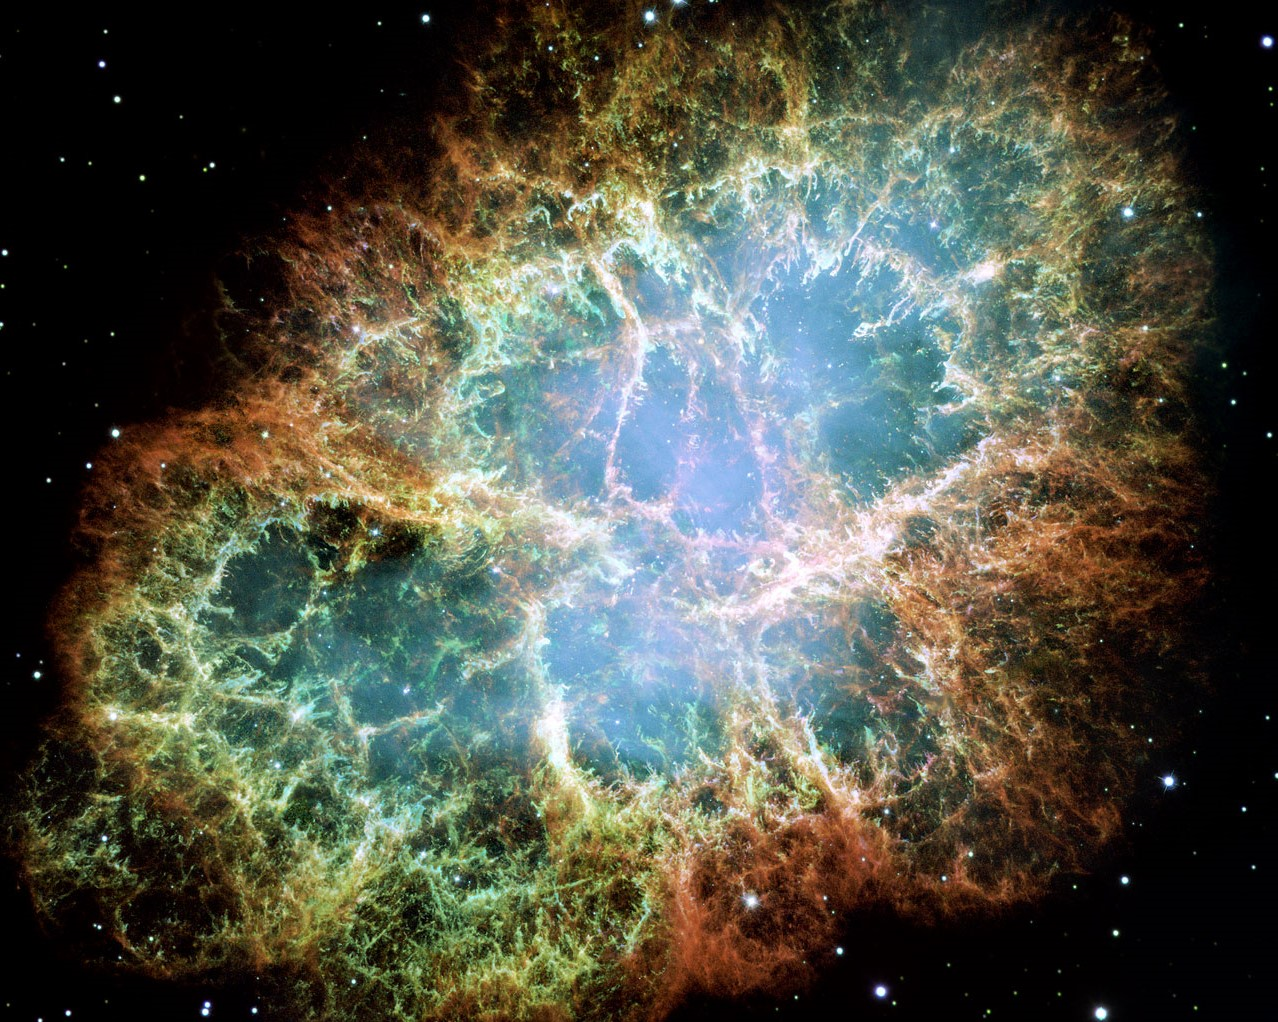
\includegraphics[width=\paperwidth, height =10cm]{../Crab.jpg}}
    \end{figure}
\end{titlepage}

%%%%%%%%%%%%%%%%%%%%%%%
\tableofcontents


%%%%%%%%%%%%%%%%%%%%%%%%%%%%%%%%%%%%% Part 1
\part{Ring Theory}

%%%%%%%%%%%%%%%%%%%%%% Chapter 1.1
\chapter{Definition of $\catname{Ring}$}

In this chapter we define the category of rings, $\catname{Ring}$, and basic properties of rings.

\section{Definition and First Examples}

We define rings (and later modules) by `decorating' abelian groups with additional data. In number systems we wish to multiply elements, and for this multiplication to `preserve' addition in some precise sense; examples are $\Z, \Q,\R,\C,\Q_p,...$. We begin by studying the structure of homomorphisms of abelian groups. Recall if $G,H$ are abelian groups, then $\Hom_{\catname{Ab}}(G,H)$ is also an abelian group. In particular, $\mathbf{End}_{\catname{Ab}}(G)$ is an abelian group, and more. Under composition $\mathbf{End}_{\catname{Ab}}(G)$ has the form of a monoid, such that the monoidal structure preserves the abelian structure - this is precisely the notion of a ring.

\begin{defn}[Ring]
    A \textbf{ring} $(R,+,\cdot)$ is an abelian group $(R,+)$ endowed with a binary operation $\cdot$ and an element $1_R \in R$ such that \begin{itemize}
        \item $\forall r,s,t \in R; (r\cdot s)\cdot t = r\cdot (s\cdot t)$ 
        \item $\forall r \in R;r\cdot 1_R = r = 1_R\cdot r$
        \item $\forall r,s,t \in R: (r+s)\cdot t = r\cdot t + s\cdot t$ and $t\cdot (r+s) = t\cdot r + t\cdot s$
    \end{itemize}
\end{defn}

Hence we are implicitly considering rings with identity. We can define a ring structure on a trivial group $\{*\}$, through which $0 = 1$. If the monoid structure on our ring is commutative, we say the ring is commutative. Not all rings are commutative, an important example of which is of $2\times 2$ matrices over a field.

\begin{defn}
    An element $a \in R$ is a \textbf{(left-)zero-divisor} if there exists $b \neq 0$ in $R$ for which $ab = 0$.
\end{defn}

Right-zero-divisors are defined similarly. $0$ is always a zero divisor in nonzero rings, so the zero ring is the only ring without zero-divisors.

\begin{prop}
    In a ring $R$, $a \in R$ is not a left- (resp., right-) zero-divisor if and only if left (resp., right) multiplication by $a$ is an injective function $R\rightarrow R$.
\end{prop}

In the case where all non-zero elements are such, we have the following definition:

\begin{defn}
    An \textbf{integral domain} is a nonzero commutative ring $R$ (with $1$) such that $$\forall a,b \in R:ab = 0\implies a =0\text{ or }b=0$$
\end{defn}

Further non-zero elements in $\Q,\R,\C$ satisfy an even nicer property:

\begin{defn}
    An element $u \in R$ is a \textbf{left-(resp.,right-)unit} if $\exists v\in R$ such that $uv = 1$ (resp. $vu = 1$). \textbf{Units} are two-sided units.
\end{defn}

\begin{prop}
    In a ring $R$: \begin{itemize}
        \item $u$ is a left-(resp., right-) unit if and only if left- (resp., right-) multiplication by $u$ is a surjective function $R\rightarrow R$.
        \item the inverse of a two-sided unit is unique
        \item two-sided units form a group under multiplication.
    \end{itemize}
\end{prop}


\begin{defn}
    A \textbf{division ring} is a ring in which every nonzero element is a two-sided unit.
\end{defn}

If the ring is also commutative with $1$ we say it is a \textbf{field}. Fields are always integral domain, but the converse is not in general true. The following is a special case where it is:

\begin{prop}
    Assume $R$ is a finite commutative ring; then $R$ is an integral domain if and only if it is a field.
\end{prop}

\section{Polynomial Rings}

\begin{defn}
    Let $R$ be a ring. A \textbf{polynomial} $f(x)$ in the \textbf{indeterminate} $x$ and with coefficients in $R$ is a finite linear combination of nonnegative powers of $x$ with coefficients in $R$: \begin{equation*}
        f(x) = \sum_{i\geq 0 }a_ix^i
    \end{equation*}
    where all $a_i \in R$ and we require $a_i = 0$ for $i \gg 0$. Two polynomials $f(x) = \sum_{i\geq 0}a_ix^i$ and $g(x) = \sum_{i\geq 0}b_ix^i$ are equal if and only if $a_i = b_i$ for all $i$. It is equipped with operations \begin{equation*}
        f(x) + g(x) := \sum_{i\geq0}(a_i+b_i)x^i
    \end{equation*}
    and \begin{equation*}
        f(x)\cdot g(x) := \sum_{k\geq 0}\sum_{i+j=k}a_ib_jx^{k}
    \end{equation*}
\end{defn}

The \textbf{degree} of a non-zero polynomial $f(x) = \sum_{i\geq 0}a_ix^i$ is $\max_n\{n:a_n\neq 0\}$ if $f(x) \neq 0$, and we define $\deg 0$ to either be $-\infty$, or simply don't define it. We can define polynomial rings in finitely many indeterminates iteratively. We can also define a ring of polynomials in countably many indeterminates, $R[x_1,x_2,...]$, as well as the ring of formal power series, $R[[x]]$.

\section{Monoid Rings}

Given a monoid $(M,\cdot)$ and a ring $R$, we can obtain a new ring $R[M]$ as follows. Elements of $R[M]$ are formal linear combinations \begin{equation*}
    \sum_{m\in M}a_m\cdot m
\end{equation*}
where $a_m \in R$ and $a_m \neq 0$ for at most finitely many summands. Addition is as before, and multiplication is given by \begin{equation*}
    \left(\sum_{m\in M}a_m\cdot m\right)\cdot \left(\sum_{m \in M}b_m\cdot m\right) = \sum_{m \in M}\sum_{m_1m_2 = m}(a_{m_1}b_{m_2})\cdot m
\end{equation*}





%%%%%%%%%%%%%%%%%%%%%% Chapter 1.2
\chapter{The Category $\catname{Ring}$}


\section{Ring Homomorphisms}

If $R,S$ are rings, a function $\varphi:R\rightarrow S$ is a ring homomorphism if it preserves both operations and the identity element. It then follows that rings form a category, with ring homomorphisms as morphisms. We denote this category by $\catname{Ring}$. The zero-ring is final in $\catname{Ring}$, but it has no maps out of it to non-zero rings.

$\catname{Ring}$ does have initial objects, namely the ring of integers $\Z$.

\section{Universal Property of Polynomial Rings}

Let $A = \{a_1,...,a_n\}$ be a set of order $n$. Consider the category whose objects are pairs $(j,R)$, where $R$ is a commutative ring and $j:A\rightarrow R$. Morphisms are commutative diagram (explicitly we are looking at a comma category). For example $(i,\Z[x_1,...,x_n])$ is an object in this category where $i:A\rightarrow \Z[x_1,...,x_n]$ sends $a_k$ to $x_k$. The pair $(i,\Z[x_1,...,x_n])$ is in fact initial in this category.

\begin{eg}
    More generally, let $\alpha:R\rightarrow S$ be a fixed ring homomorphism, and let $s \in S$ be an element commuting with $\alpha(R)$. Then there is a unique ring homomorphism $\overline{\alpha}:R[x]\rightarrow S$ extending $\alpha$ and sending $x$ to $s$.
\end{eg}

In particular this gives an evaluation map for polynomials over commutative rings, $R[x]\rightarrow R$.


\section{Monomorphisms and Epimorphisms}

The kernel of a homomorphism of rings is not in general a subring, and in fact is only a subring if it is the whole ring and we are mapping to the zero ring. However we do have the nice property that a ring homomorphism is a monomorphism if and only if its kernel is trivial.

However, unlike in group epimorphisms need not be surjective in $\catname{Ring}$. For example the monomorphism $\iota:\Z\hookrightarrow \Q$ is also an epimorphism. This also provides an example of a map which is both a monomorphism and an epimorphism but not an isomorphism.


Further, on a categorical note, $\catname{Ring}$ has finite products.

\section{Endomorphism Rings}

For an abelian group $G$ we return to the endomorphism group $\mathbf{End}_{\catname{Ab}}(G)$. Under composition we can endow this group with a ring structure. For example, $\mathbf{End}_{\catname{Ab}}(\Z)\cong \Z$ as rings. The group of units in these rings is simply $\mathbf{Aut}_{\catname{Ab}}(G)$.

Every ring $R$ interacts with the ring of endomorphisms of the underlying abelian group through left and right multiplication.

\begin{prop}
    Let $R$ be a ring. Then the function $r\mapsto L_r$ is an injective ring homomorphism $$\lambda:R\rightarrow \mathbf{End}_{\catname{Ab}}(R)$$
\end{prop}

The right multiplication map is almost a ring homomorphism, in the sense that composition reverses the order of multiplication, which means it is a ring homomorphism in the case of a commutative $R$.




%%%%%%%%%%%%%%%%%%%%%% Chapter 1.3
\chapter{Ideals and Quotient Rings}

\section{Ideals}

\begin{defn}
    Let $R$ be a ring. A subgroup $I$ of $(R,+)$ is a \textbf{left-ideal} of $R$ if $rI \subseteq I$ for all $r \in R$; that is $$\forall r\in R,\forall a \in I:ra \in I$$ it is a \textbf{right-ideal} if $Ir \subseteq I$ for all $r \in R$; that is $$\forall r \in R,\forall a \in I:ar \in I$$
    A \textbf{two-sided ideal} is a subgroup $I$ which is both a left- and a right-ideal.
\end{defn}

Kernels and two-sided ideals in $\catname{Ring}$ are equivalent.


\section{Quotients}

For $I$ a two-sided ideal of $R$ we can form the quotient ring $R/I$, with natural multiplication and addition. This satisfies the suitable universal property as in the group homomorphisms case. The structure on $R/I$ is completely forced by the requirement that the natural projection $\pi:R\rightarrow R/I$ is a ring homomorphism. 

The fact that $\Z$ is initial in $\catname{Ring}$ prompts a natural definition: for a ring $R$, let $f:\Z\rightarrow R$ be the unique ring homomorphism. Then $\ker f = n\Z$ for a well-defined nonnegative integer $n$ determined by $R$.

\begin{defn}
    The \textbf{characteristic} of $R$ is this nonnegative integer $n$.
\end{defn}

Thus, the characteristic of $R$ is $n > 0$ if the order of $1_R$ as an element of $(R,+)$ is finite, while the characteristic is $0$ if the order of $1_R$ is $\infty$.

Our universal property for quotients is as follows:

\begin{thm}
    Let $I$ be a two-sided ideal of a ring $R$. Then for every ring homomorphism $\varphi:R\rightarrow S$ such that $I \subseteq \ker \varphi$, there exists a unique ring homomorphism $\widetilde{\varphi}:R/I\rightarrow  S$ so that the diagram
    \begin{center}
        \begin{tikzpicture}[baseline= (a).base]
\node[scale=1] (a) at (0,0){
 \begin{tikzcd}
	R && S \\
	& {R/I}
	\arrow["\varphi", from=1-1, to=1-3]
	\arrow["\pi"', from=1-1, to=2-2]
	\arrow["{\widetilde{\varphi}}"', dashed, from=2-2, to=1-3]
\end{tikzcd} 
};
\end{tikzpicture}
\end{center}
commutes.
\end{thm}


From this result we can further derive a decomposition of ring homomorphisms:

\begin{thm}
    Every ring homomorphism $\varphi:R\rightarrow S$ may be decomposed as follows:
    \begin{center}
\begin{tikzpicture}[baseline= (a).base]
\node[scale=1] (a) at (0,0){
 \begin{tikzcd}
	R & {R/\ker\varphi} & {\ran \varphi} & S
	\arrow["\pi"', two heads, from=1-1, to=1-2]
	\arrow["\iota"', hook, from=1-3, to=1-4]
	\arrow["\sim", dashed, from=1-2, to=1-3]
	\arrow["\varphi", curve={height=-18pt}, from=1-1, to=1-4]
	\arrow["{\widetilde{\varphi}}"', dashed, from=1-2, to=1-3]
\end{tikzcd} 
};
\end{tikzpicture}
\end{center}
    where the isomorphism $\widetilde{\varphi}$ is induced by $\varphi$.
\end{thm}

We immediately obtain the first isomorphism theorem as a corollary:

\begin{cor}
    Suppose $\varphi:R\rightarrow S$ is a surjective ring homomorphism. Then $S\cong R/\ker \varphi$.
\end{cor}

We also have the correspondence of ideals of $R/I$ with ideals of $R$ containing $I$, given by the natural projection map. We also have the following consequence:

\begin{prop}
    Let $I$ be a two-sided ideal of a ring $R$ and let $J$ be a two-sided ideal of $R$ containing $I$. Then $J/I$ is a two-sided ideal of $R/I$, and \begin{equation*}
        \frac{R/I}{J/I}\cong R/J
    \end{equation*}
\end{prop}


\section{Operations on Ideals}

Let $a \in R$. Then $Ra$ (resp. $aR$) is a left- (resp. right-) ideal of $R$. In the commutative case these coincide and are denoted $(a)$, the \textbf{principal ideal generated by $a$}.

If $\{I_{\alpha}\}_{\alpha \in A}$ is a family of ideals of a ring $R$, then the sum $\sum_{\alpha}I_{\alpha}$ is an ideal of $R$. In the case of a family of principle ideals we have $$(a_{\alpha})_{\alpha \in A} := \sum_{\alpha \in A}(a_{\alpha})$$


\begin{defn}
    A commutative ring $R$ is \textbf{Noetherian} if every ideal of $R$ is finitely generated.
\end{defn}

\begin{defn}
    An integral domain $R$ is a \textbf{Principal Ideal Domain (PID)} if every ideal of $R$ is principal.
\end{defn}

$\Z$ is a well-known example of a PID. If $k$ is a field, the ring of polynomials $k[x]$ is a PID, but $\Z[x]$ is not.

The intersection of an arbitrary family of ideals is again an ideal, and for two ideals $I,J \subseteq R$, their product $IJ$ is the ideal generated by all products $ij$ for $i \in I$ and $j \in J$.


\section{Quotients of Polynomial Rings}

Let $R$ be a nonzero ring and let $f \in R[x]$ be a monic polynomial. Supposing that $f$ is monic allows us to \textbf{divide} by $f(x)$, with remainder. That is for any $g(x) \in R[x]$, there exist $q(x), r(x) \in R[x]$ such that $g(x) = f(x)q(x) + r(x)$ where $\deg r(x) < \deg f(x)$. Further the quotient and remainder polynomials are unique.

Looking at this in another way we have that all cosets in $R[x]/(f(x))$ are represented by polynomials of degree less than $\deg f(x)$. We can then view the quotient as $R^{\oplus \deg f(x)}$ with a naturally endowed ring structure. In particular as abelian groups $R[x]/(f(x)) \cong R^{\oplus \deg f(x)}$. If $\deg f(x) = 1$ then these ring structures are isomorphic, but for degrees 2 or greater we already can find interesting distinct structures.


\section{Prime and Maximal Ideals}

\begin{defn}
    Let $I \neq R$ be an ideal of commutative ring $R$. \begin{itemize}
        \item $I$ is a \textbf{prime ideal} if $R/I$ is an integral domain
        \item $I$ is a \textbf{maximal ideal} if $R/I$ is a field.
    \end{itemize}
\end{defn}

\begin{prop}
    Let $I \neq R$ be a proper ideal of a commutative ring $R$. Then \begin{itemize}
        \item $I$ is prime if and only if for all $a,b \in R$, $ab \in I$ implies $a \in I$ or $b \in I$. Equivalently, \begin{equation*}
                (ab) \subseteq I\implies ((a) \subseteq I)\lor (b) \subseteq I)
        \end{equation*}
        \item $I$ is maximal if and only if for all ideals $J$ of $R$, \begin{equation*}
                I \subseteq J\implies (I = J\lor J = R)
        \end{equation*}
    \end{itemize}
\end{prop}


Note that maximal implies prime, but in general the converse is false.

\begin{prop}
    Let $I$ be an ideal of a commutative ring $R$. If $R/I$ is finite then $I$ is prime if and only if it is maximal.
\end{prop}

For PIDs we have equivalence:

\begin{prop}
    Let $R$ be a PID, and let $I$ be a nonzero ideal in $R$. Then $I$ is prime if and only if it is maximal.
\end{prop}

\begin{defn}
    The \textbf{Krull dimension} of a commutative ring $R$ is the length of the longest chain of prime ideals in $R$.
\end{defn}

Hence all PIDs have dimension $1$, so they correspond to curves in algebraic geometry.


%%%%%%%%%%%%%%%%%%%%%% Chapter 1.4
\chapter{Chain Conditions and Factorization}

\section{Prime and irreducible elements}

Let $R$ be a commutative ring. We say that $a,b \in R$ are \textbf{associates} if $(a) = (b)$.

\begin{lem}
    Let $a,b$ be nonzero elements of an integral domain $R$. Then $a$ and $b$ are associated if and only if $a = ub$ for $u$ a unit in $R$.
\end{lem}

\begin{defn}
    Let $R$ be an integral domain. \begin{itemize}
        \item An element $a \in R$ is \textbf{prime} if the ideal $(a)$ is prime.
        \item An element $a \in R$ is \textbf{irreducible} if $a$ is not a unit and $$a=bc \implies (b \in R^{\times}\lor c \in R^{\times})$$
    \end{itemize}
\end{defn}

The definition of irreducible is equivalent to the statement that $(a)$ is maximal among proper principal ideals. These notions are not in general equivalent, though in an integral domain primality implies irreducibility.

\begin{lem}
    Let $R$ be an integral domain, and let $a \in R$ be a nonzero prime element. Then $a$ is irreducible.
\end{lem}

\section{Factorization into Irreducibles}

\begin{defn}
    Let $R$ be an integral domain. An element $r \in R$ has a \textbf{factorization} into irreducibles if there exist irreducible elements $q_1,...,q_n$ such that $r = q_1\cdots q_n$.
\end{defn}
This factorization is said to be unique if the elements $q_i$ are determined by $r$ up to order and associates.

\begin{defn}
    An integral domain $R$ is a domain with factorizations if every nonzer nonunit element $r \in R$ has a factorization into irreducibles.
\end{defn}

\begin{defn}
    An integral domain $R$ is a \textbf{unique factorization domain (UFD)}, if every nonzero, nonunit element $r \in R$ has a unique factorization into irreducibles.
\end{defn}

Existence of factorizations is implies by an ascending chain condition:

\begin{prop}
    Let $R$ be an integral domain, and let $r$ be a nonzero, nonunit element of $R$. Assume that every ascending chain of principal ideals $$(r) \subseteq (r_1) \subseteq (r_2) \subseteq \cdots$$ 
    stabilizes. Then $r$ has a factorization into irreducibles.
\end{prop}

\begin{cor}
    Let $R$ be a Noetherian domain. Then factorizations exist in $R$.
\end{cor}

However Noetherian domains are not necessary for factorizations. For example $\Z[x_1,x_2,x_3,...]$ does have factorizations but is not a Noetherian ring.

%%%%%%%%%%%%%%%%%%%%%% Chapter 1.5
\chapter{UFDs, PIDs, Euclidean Domains}


\section{Irreducible Factors and GCDs}

In a UFD all elements determine a multiset of irreducible factors, determined up to the associate relation.

\begin{lem}
    Let $R$ be a UFD, and let $a,b,c$ be nonzero elements of $R$. Then \begin{itemize}
        \item $(a) \subseteq (b) \iff$ the multiset of irreducible factors of $b$ is contained in the multiset of irreducible factors of $a$.
        \item $a$ and $b$ are associates if and only if the two multisets coincide.
        \item the irreducible factors of a product $bc$ are the collection of all irreducible factors of $b$ and of $c$.
    \end{itemize}
\end{lem}

\begin{defn}
    Let $R$ be an integral domain, and let $a,b \in R$. An element $d \in R$ is a \textbf{greatest common divisor} of $a$ and $b$ if $(a,b) \subseteq (d)$ and $(d)$ is the smallest principal ideal in $R$ with this property.
\end{defn}

GCDs need not exist in general, but they do in UFDs.

\begin{lem}
    Let $R$ be a UFD, and let $a,b$ be nonzero elements of $R$. Then $a,b$ have a greatest common divisor.
\end{lem}


\section{Characterization of UFDs}

\begin{lem}
    Let $R$ be a UFD, and let $a$ be an irreducible element of $R$. Then $a$ is prime.
\end{lem}

\begin{thm}
    An integral domain $R$ is a UFD if and only if \begin{itemize}
        \item the a.c.c. for principal ideals holds in $R$ and 
        \item every irreducible element of $R$ is prime
    \end{itemize}
\end{thm}

The PID condition is explicitly stronger than the UFD condition in that all PIDs are UFDs.

\begin{prop}
    If $R$ is a PID, then it is a UFD.
\end{prop}

Of course there are many UFDs which are not PIDs, evidenced by the fact that there are even UFDs which are not Noetherian rings,and all PIDs are Noetherian.

An even stronger requirement than PID is that of being a \textbf{Euclidean domain}. For the purpose of this discussion, a \textbf{valuation} on an integral domain $R$ is a function $v:R\backslash\{0\}\rightarrow \Z^{\geq 0}$.

\begin{defn}
    A \textbf{Euclidean valuation} on an integral domain $R$ is a valuation satisfying the following property: for all $a \in R$ and all nonzero $b \in R$, there exists $q,r \in R$ such that $$a  =qb+r$$
    with either $r = 0$ or $v(r) < v(b)$. An integral domain $R$ is a \textbf{Euclidean domain} if it admits a Euclidean valuation.
\end{defn}

\begin{prop}
    Let $R$ be a Euclidean domain. Then $R$ is a PID.
\end{prop}

One excellent feature of Euclidean domains is a Euclidean algorithms. The key lemma on which the algorithm is based in the following fact: 

\begin{lem}
    Let $a = bq+r$ in a ring $R$. Then $(a,b) = (b,r)$.
\end{lem}

That is the set of common divisors of $a,b$ and the set of common divisors of $b,r$ coincide.

\begin{cor}
    Assume $a  =bq+r$. Then $a,b$ have a gcd if and only if $b,r$ have a gcd, and in this case $gcd(a,b) = gcd(b,r)$.
\end{cor}


%%%%%%%%%%%%%%%%%%%%%% Chapter 1.6
\chapter{Unique Factorization in Polynomial Rings}

After necessary work we aim to show that $R[x]$ is a UFD if $R$ is.


\section{Primitivity and Content; Gauss's Lemma}

Observe that every ideal $I$ of $R$ generates an ideal of $R[X]$, \begin{equation*}
    IR[X] := \{a_0+a_1X+\cdots+a_dX^d \in R[X]:\forall i,a_i \in I\}
\end{equation*}

\begin{lem}
    Let $R$ be a ring, and let $I$ be an ideal of $R$. Then \begin{equation*}
        R[X]/IR[X] \cong (R/I)[X]
    \end{equation*}
\end{lem}

\begin{cor}
    If $I$ is a prime ideal of $R$, then $IR[X]$ is a prime in $R[X]$.
\end{cor}

\begin{defn}
    Let $R$ be a commutative ring, and let $f = a_0+a_1x+\cdots+a_dx^d \in R[x]$ be a polynomial. \begin{itemize}
        \item $f$ is \textbf{very primitive} if for all prime ideals $\mathfrak{p}$ of $R$, $f \notin \mathfrak{p}R[x]$
        \item $f$ is \textbf{primitive} if for all principal prime ideals $\mathfrak{p}$ of $R$, $f \notin \mathfrak{p}R[x]$
    \end{itemize}
\end{defn}

Very primitive polynomials are primitive, but the converse does not hold in general, even in UFDs.

\begin{lem}
    Let $R$ be a commutative ring. Then for $f,g \in R[x]$, $$fg\text{ is primitive}\iff\text{both $f$ and $g$ are primitive}$$
\end{lem}

\begin{lem}
    Let $R$ be a commutative ring and $f = a_0+a_1x+\cdots+a_dx^d \in R[x]$ as above. \begin{itemize}
        \item $f$ is very primitive if and only if $(a_0,...,a_d) = (1)$
        \item If $R$ is a UFD, then $f$ is primitive if and only if $\text{gcd}(a_0,...,a_d) = 1$
    \end{itemize}
\end{lem}

\begin{defn}
    Let $R$ be a UFD. The \textbf{content} of a nonzero polynomial $f \in R[x]$, denoted $\text{cont}_f$, is the gcd of its coefficients.
\end{defn}

Thus $f$ is primitive precisely when $(\text{cont}_f) = (1)$.

\begin{lem}
    Let $R$ be a UFD, and let $f \in R[x]$. Then \begin{itemize}
        \item $(f) = (\text{cont}_f)(\underline{f})$, where $\underline{f}$ is primitive
        \item if $(f) = (c)(g)$, with $c \in R$ and $g$ primitive, then $(c) = (\text{cont}_f)$.
    \end{itemize}
\end{lem}

\begin{prop}[Gauss's Lemma]
    Let $R$ be a UFD, and let $f,g \in R[x]$. Then \begin{equation*}
        (\text{cont}_{fg}) = (\text{cont}_f)(\text{cont}_g)
    \end{equation*}
\end{prop}

\begin{cor}
    Let $R$ be a UFD, and let $f,g \in R[x]$. Assume $(f) \subseteq (g)$. Then $(\text{cong}_f) \subseteq (\text{cont}_g)$.
\end{cor}

\section{The Field of Fractions}

The Field of Fractions is a special case of a universal construction known as localization. For an integral domain $R$, its field of fractions is the pair $(i,K(R))$ where $i:R\rightarrow K(R)$ is an injective ring homomorphism and $K(R)$ is a field, and this pair is initial with this property. Thus $K(R)$ is in a way the `smallest field containing $R$'.


An explicit construction of $K(R)$ is given by $R\times (R\backslash\{0\})/\sim$, where $(a,b)\sim (d,c)$ if and only if $ac = bd$. Multiplication and addition are done as in $\Q$ (in particular, $\Q$ is the field of fractions of $\Z$).

\begin{defn}
    The field of \textbf{rational functions} with coefficients in $R$ is the field of fractions of the ring $R[x]$. This field is denoted $R(x)$.
\end{defn}

We are now in a position to prove the following:
\begin{thm}
    Let $R$ be a UFD, then $R[x]$ is a UFD.
\end{thm}

By an immediate induction we have that $\Z[x_1,...,x_n]$ and $k[x_1,...,x_n]$ are UFDs. However, $R[[x]]$ is not necessarily a UFD even if $R$ is.

We aim to verify that $R[x]$ satisfies the a.c.c. on principal ideals, and that every irreducible element in $R[x]$ is prime, provided $R$ is a UFD. We aim to reduce these questions to $K(R)[x]$.

\begin{lem}
    Let $R$ be a UFD and let $K$ be its field of fractions. For nonzero $f,g \in R[x]$, denote by $(f), (g)$ the principal ideals $fR[x],gR[x]$ in $R[x]$, and denote by $(f)_K,(g)_K$ the principal ideals $fK[x],gK[x]$ in $K[x]$. Assume \begin{itemize}
        \item $(\text{cont}_g) \subseteq (\text{cont}_f)$ and 
        \item $(g)_K \subseteq (f)_K$
    \end{itemize}
    Then $(g) \subseteq (f)$.
\end{lem}

\begin{prop}
    Let $R$ be a UFD, and let $f \in R[x]$ be a nonconstant, irreducible polynomial. Then $f$ is irreducible as an element of $K(R)[x]$.
\end{prop}

\begin{cor}
    Let $R$ be a UFD and let $f \in R[x]$ be a nonconstant polynomial. Then $f$ is irreducible in $R[x]$ if and only if it is irreducible in $K[x]$ and primitive.
\end{cor}




%%%%%%%%%%%%%%%%%%%%%%%%%%%%%%%%%%%%% Part 2
\part{Module Theory}

%%%%%%%%%%%%%%%%%%%%%% Chapter 2.1
\chapter{Intro to Modules over a Ring}

The category $\catname{Ring}$ fails to satisfy many nice properties, such as how kernels and cokernels behave. Modules will fix a majority of these issues. If $R$ is a ring and $I \subseteq R$ is a two-sided ideal, then all three structures $R, I,$ and $R/I$ will be modules over $R$.

\section{Definition of (left-)$R$-modules}

A left-$R$-module $M$ is simply an abelian group $(M,+)$ along with a ring action given by a homomorphism of rings $$\sigma:R\rightarrow \mathbf{End}_{\catname{Ab}}(M)$$

\begin{prop}
    The datum of a homomorphism $\sigma$ as above is precisely the same as the datum of a function $$\rho:R\times M\rightarrow M$$ 
    satisfying the following requirements: $\forall r,s \in R,\forall m,n \in M$
    \begin{itemize}
        \item $\rho(r,m+n) = \rho(r,m)+\rho(r,n)$
        \item $\rho(r+s,m) = \rho(r,m) + \rho(s,m)$
        \item $\rho(rs,m) = \rho(r,\rho(s,m))$
        \item $\rho(1,m) = m$
    \end{itemize}
\end{prop}

We can define right-$R$-modules analogously, viewing a right-$R$-module as a left-$R^{op}$-module structure. These issues become immaterial if $R$ is commutative. Then the identity $R\rightarrow R^{op}$ is an isomorphism, and left-modules/right-modules are identical concepts.

\section{The Category $\catname{R-mod}$}

As a first example we note that $\Z-\catname{mod}\cong \catname{Ab}$ are equivalent categories in a natural way.

A homomorphism of $R$-modules is a homomorphism of abelian groups which is compatible with the module structure. The set $\mathbf{Hom}_R(M,N)$ has the structure of an abelian group for any $R$-modules $M$ and $N$.

Given a ring homomorphism $\alpha:R\rightarrow S$, we can induce an $R$-module structure on $S$. Further if $\alpha(R)$ also lands in the center of $S$ we define the following notion.

\begin{defn}
    Let $R$ be a commutative ring. An \textbf{$R$-algebra} is a ring homomorphism $\alpha:R\rightarrow S$ such that $\alpha(R)$ is contained in the center of $S$.
\end{defn}

An $R$-algebra $S$ is a \textbf{division algebra} if $S$ is a division ring. This gives us another category $\catname{R-Alg}$. Further, $\Z-\catname{Alg}$ is equivalent to $\catname{Ring}$.

Canonical examples are the polynomial rings $R[x_1,...,x_n]$ and their $R$-algebras.

The category of $R$-modules has a zero object given by inducing a module structure on the trivial group, $0$. 

Now, if $R$ is commutative, $\mathbf{Hom}_R(M,N) \in R-\catname{mod}$. 


\section{Submodules and Quotients}

A \textbf{submodule} $N$ of an $R$-module $M$ is a subgroup preserved by the action of $R$. Equivalently $N$ is an $R$-module with the natural inclusion $N \subseteq M$ being an $R$-module homomorphism. Both the kernel and image of a homomorphism of $R$-modules are submodules.

If $N$ is a submodule of $M$ we can define the quotient $M/N$ of abelian groups, and it can then be shown that their is a unique module structure on $M/N$ for which $\pi:M\rightarrow M/N$ is an $R$-module homomorphism.

\begin{rmk}
    If $R$ is not commutative and $I$ is a left-ideal, then the quotient $R/I$ need not be defined as a ring, but it is defined as a left-module.
\end{rmk}


\begin{thm}
    Let $N$ be a submodule of an $R$-module $M$. Then for every homomorphism of $R$-modules $\varphi:M\rightarrow P$ such that $N \subseteq \ker \varphi$ there exists a unique homomorphism of $R$-modules $\widetilde{\varphi}:M/N\rightarrow P$ so that the diagram 
    \begin{center}
\begin{tikzpicture}[baseline= (a).base]
\node[scale=1] (a) at (0,0){
 \begin{tikzcd}
	M && N \\
	& {M/N}
	\arrow["\varphi", from=1-1, to=1-3]
	\arrow["\pi"', two heads, from=1-1, to=2-2]
	\arrow["{\widetilde{\varphi}}"', dashed, from=2-2, to=1-3]
\end{tikzcd} 
};
\end{tikzpicture}
\end{center}
commutes.
\end{thm}

As in previous cases we have a one-to-one correspondence between kernels of $R$-module homomorphisms out of $M$ and submodules of $M$. Further, every monomorphism in $R$-mod is a kernel.


\begin{thm}
    Every $R$-module homomorphism $\varphi:M\rightarrow M'$ may be decomposed as follows: 
    \begin{center}
\begin{tikzpicture}[baseline= (a).base]
\node[scale=1] (a) at (0,0){
  \begin{tikzcd}
	M & {M/\ker\varphi} & \ran\varphi & {M'}
	\arrow["\varphi", curve={height=-18pt}, from=1-1, to=1-4]
	\arrow["\pi"', two heads, from=1-1, to=1-2]
	\arrow["\sim", dashed, from=1-2, to=1-3]
	\arrow["{\widetilde{\varphi}}"', dashed, from=1-2, to=1-3]
	\arrow["\iota"', hook, from=1-3, to=1-4]
\end{tikzcd}};
\end{tikzpicture}
\end{center}
    where the isomorphism $\widetilde{\varphi}$ is induced by $\varphi$.
\end{thm}

\begin{cor}
    Suppose $\varphi:M\rightarrow M'$ is a surjective $R$-module homomorphism. Then $M'\cong M/\ker \varphi$.
\end{cor}
If $N$ is a submodule of $M$ then there is a bijection between submodules of $M$ containing $N$ and submodules of $M/N$, induced by $\pi$.

\begin{prop}
    Let $N$ be a submodule of an $R$-module $M$, and let $P$ be a submodule of $R$ containing $N$. Then $P/N$ is a submodule of $M/N$ and \begin{equation*}
        \frac{M/N}{P/N}\cong M/P
    \end{equation*}
\end{prop}

\begin{prop}
    Let $N$ and $P$ be submodules of an $R$-module $M$. Then \begin{itemize}
        \item $N+P$ is a submodule of $M$
        \item $N \cap P$ is a submodule of $P$, and \begin{equation*}
                \frac{N+P}{N}\cong \frac{P}{N\cap P}
        \end{equation*}
    \end{itemize}
\end{prop}


\section{Noetherian Modules}

\begin{defn}
    An $R$-module $M$ is Noetherian if every submodule of $M$ is finitely generated.
\end{defn}

This condition is preserved through exact sequences: if $M,N,P$ are $R$-modules and $$0\rightarrow N\hookrightarrow M\twoheadrightarrow P \rightarrow 0$$
is an exact sequence, then $M$ is Noetherian if and only if both $N$ and $P$ are Noetherian.

\begin{cor}
    Every finitely sum of Noetherian modules is Noetherian.
\end{cor}

\begin{prop}
    Let $R$ be a commutative ring, and let $M$ be an $R$-module. Then the following are equivalent: \begin{enumerate}
        \item $M$ is Noetherian
        \item $M$ satisfies the a.c.c. on submodules
        \item Every nonempty family of submodules of $M$ has a maximal element with respect to incluson.
    \end{enumerate}
\end{prop}


\begin{thm}
    Let $R$ be a Noetherian ring, and let $J$ be an ideal of the polynomial ring $R[x_1,...,x_n]$. Then the ring $R[x_1,...,x_n]/J$ is Noetherian.
\end{thm}

\begin{lem}[Hilbert's Basis Theorem]
    If $R$ is Noetherian then $R[x]$ is Noetherian.
\end{lem}



%%%%%%%%%%%%%%%%%%%%%% - Appendices
\begin{appendices}
	

\end{appendices}


\end{document}


%%%%%% END %%%%%%%%%%%%%
